\subsection{Number of Contacts}
\label{subsec:data_number_of_contacts}

We calibrate the parameters for the predicted numbers of contacts from contact diaries of
over 2000 individuals from Germany, Belgium, the Netherlands and Luxembourg
\citep{Mossong2008}. Each contact diary contains all contacts an individual had
throughout one day, including information on the other person (such as age and gender)
and information on the contact. Importantly, for each contact individuals entered of
which type the contact (school, leisure, work etc.) was and how frequent the contact with
the other person is. Binning the number of contacts for very high numbers, we arrive at
the distributions of the numbers of contacts by contact type as shown in Figure~\ref{fig:n_contacts}.

\begin{figure}[ht]
    \centering
    % other contacts
    \begin{subfigure}[b]{0.3\textwidth}
        \centering
        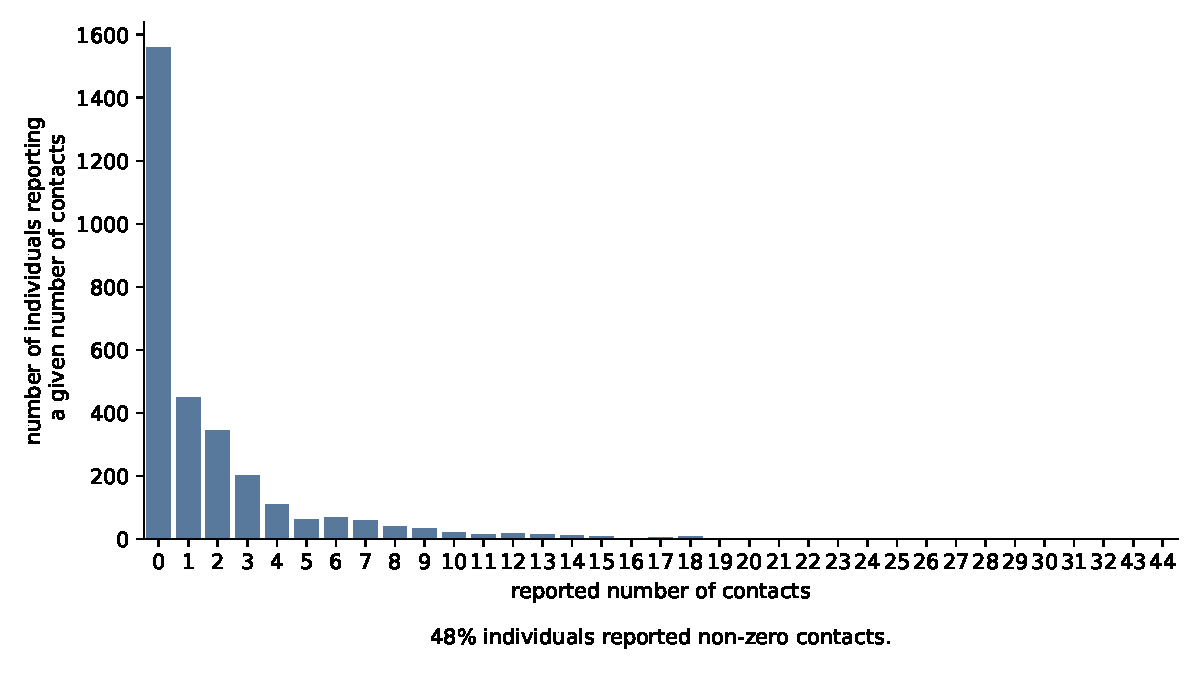
\includegraphics[width=\textwidth]{figures/results/figures/data/distributions_of_the_number_of_contacts/other_non_recurrent}
        \caption{Number of Non Recurrent Other Contacts}
        \label{fig:n_contacts_other_non_recurrent}
    \end{subfigure}
    \hfill
    \begin{subfigure}[b]{0.3\textwidth}
        \centering
        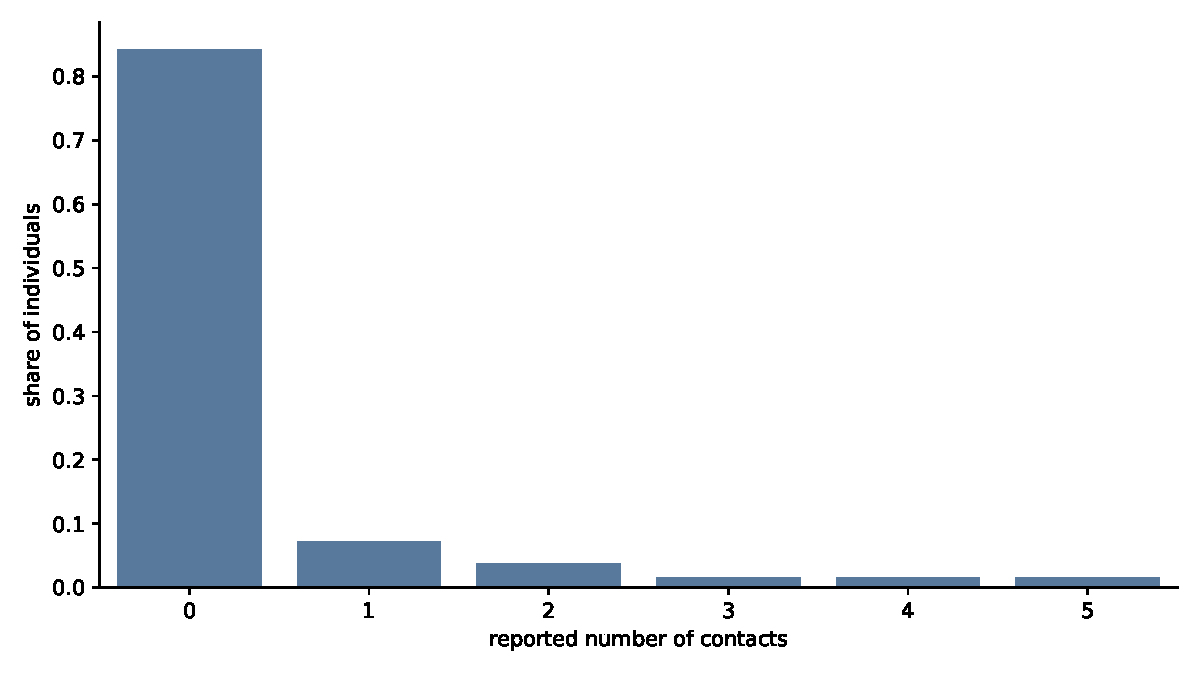
\includegraphics[width=\textwidth]{figures/results/figures/data/distributions_of_the_number_of_contacts/other_recurrent_daily}
        \caption{Number of Daily Recurrent Other Contacts}
        \label{fig:n_contacts_other_daily_recurrent}
    \end{subfigure}
    \hfill
    \begin{subfigure}[b]{0.3\textwidth}
        \centering
        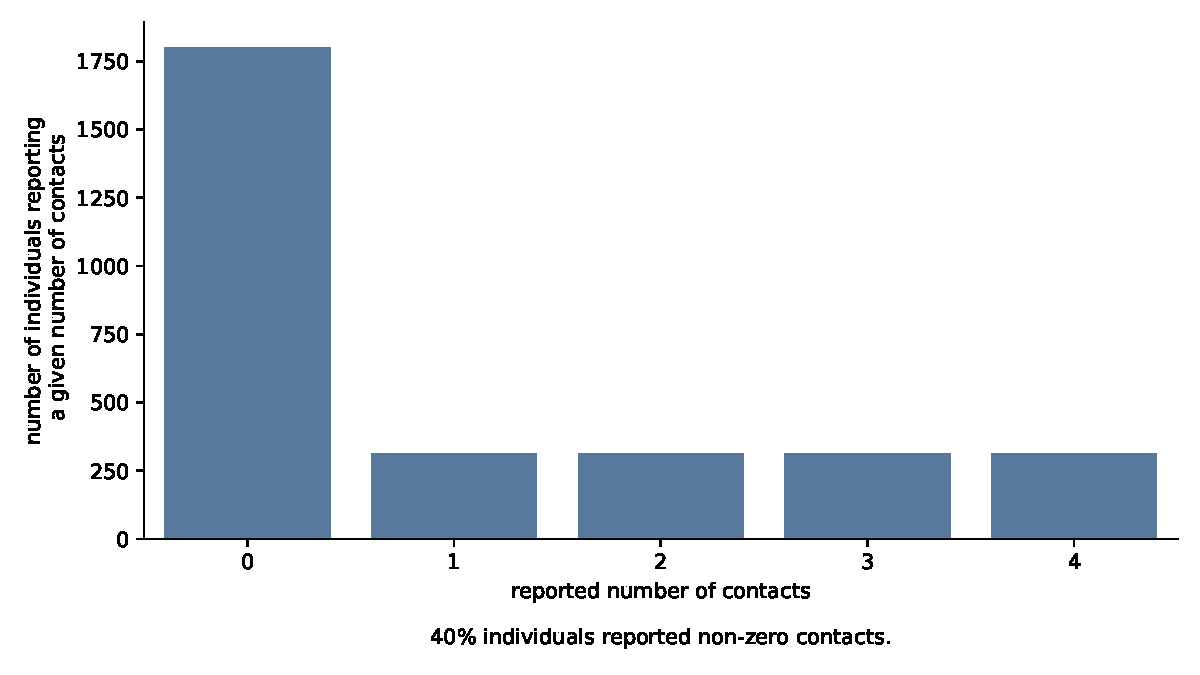
\includegraphics[width=\textwidth]{figures/results/figures/data/distributions_of_the_number_of_contacts/other_recurrent_weekly}
        \caption{Number of Weekly Recurrent Other Contacts}
        \label{fig:n_contacts_other_weekly_recurrent}
    \end{subfigure}

    \vskip3ex

    % work contacts
    \begin{subfigure}[b]{0.3\textwidth}
        \centering
        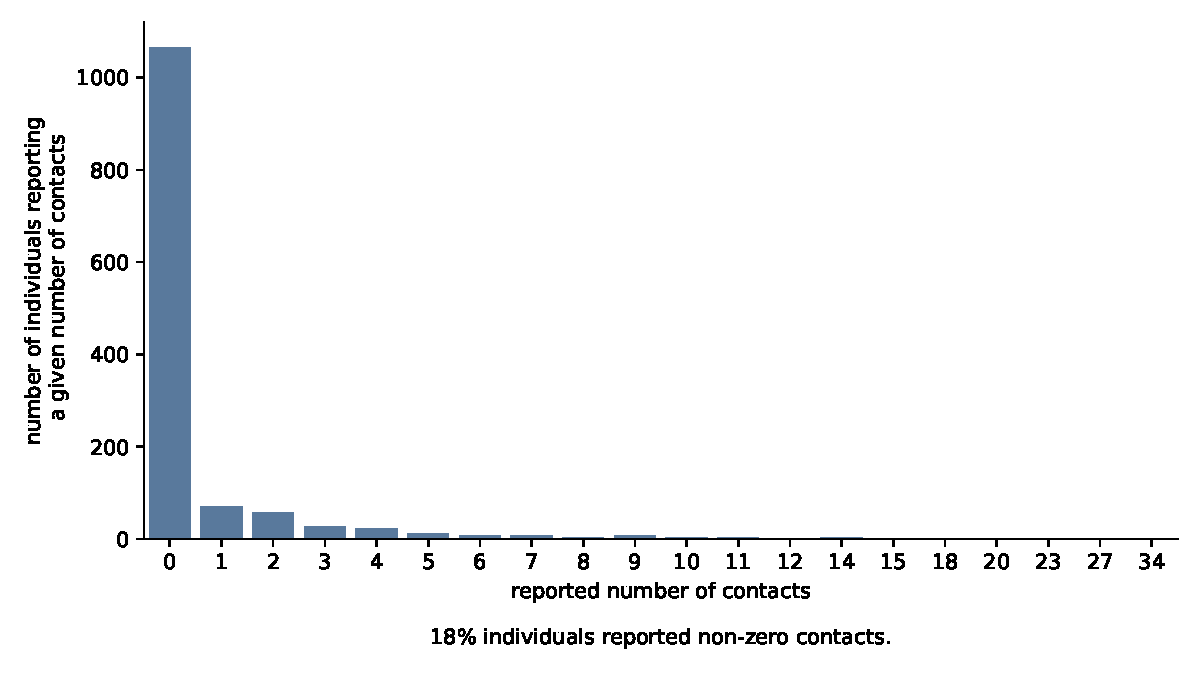
\includegraphics[width=\textwidth]{figures/results/figures/data/distributions_of_the_number_of_contacts/work_non_recurrent}
        \caption{Number of Non Recurrent Work Contacts}
        \label{fig:n_contacts_work_non_recurrent}
    \end{subfigure}
    \hfill
    \begin{subfigure}[b]{0.3\textwidth}
        \centering
        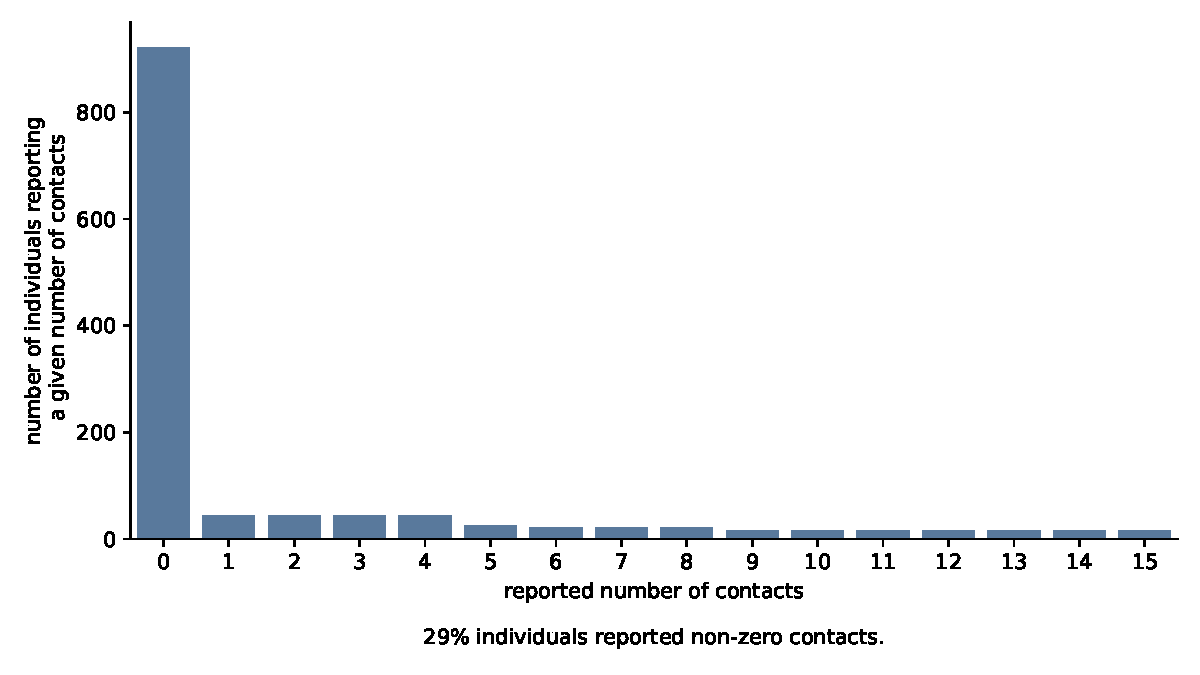
\includegraphics[width=\textwidth]{figures/results/figures/data/distributions_of_the_number_of_contacts/work_recurrent_daily}
        \caption{Number of Daily Recurrent Work Contacts}
        \label{fig:n_contacts_work_daily_recurrent}
    \end{subfigure}
    \hfill
    \begin{subfigure}[b]{0.3\textwidth}
        \centering
        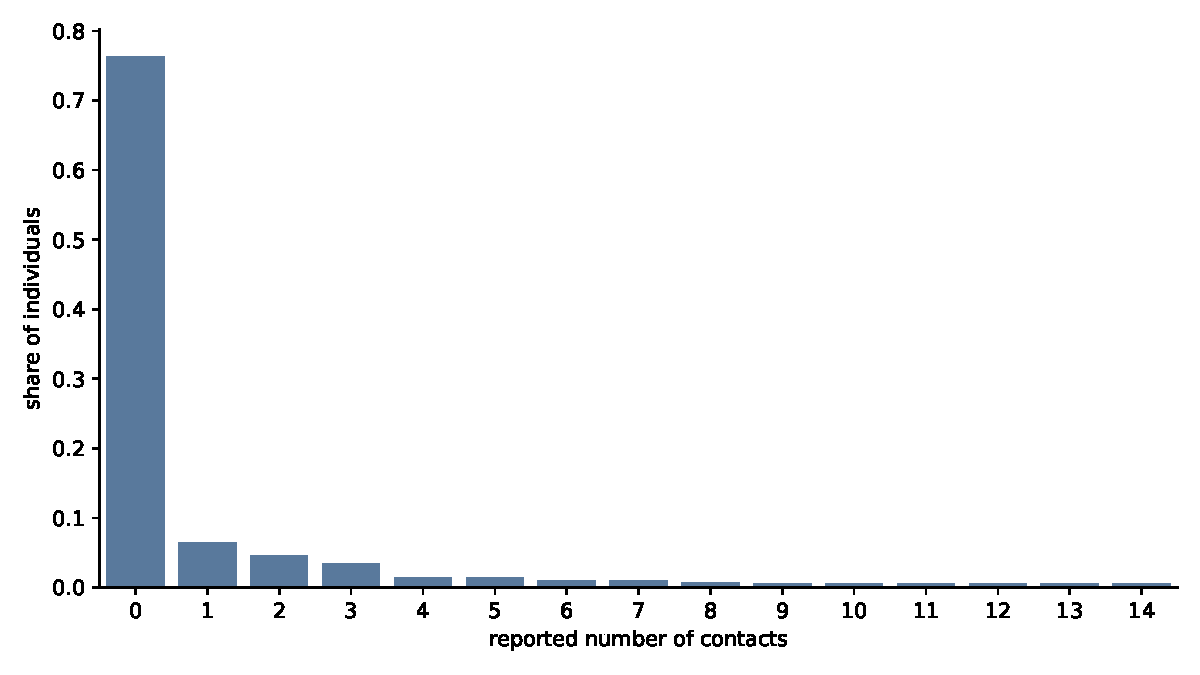
\includegraphics[width=\textwidth]{figures/results/figures/data/distributions_of_the_number_of_contacts/work_recurrent_weekly}
        \caption{Number of Weekly Recurrent Work Contacts}
        \label{fig:n_contacts_work_weekly_recurrent}
    \end{subfigure}
    \vskip3ex

    \caption{Number of Contacts of the Different Contact Types}
    \label{fig:n_contacts}
    \floatfoot{\noindent
        \textit{Note:} This figure shows the pre-pandemic number of contacts individuals
        report of different contact types.
        % non recurrent contacts
        In the model it is sampled every day which of the numbers of non recurrent
        contacts a person is planned to have. Note that the contact diaries include such
        high values that super spreading events are well possible in our model through
        non recurrent models.
        % recurrent contacts
        For recurrent contacts individuals are put into groups that meet either every day
        or on a particular week day every day. For work contacts, meetings can only take
        place on work days.
        % reductions that can happen
        The pre-pandemic number of contacts with transmission potential is reduced by
        policies, seasonality and individual responses to events such as
        receiving a positive rapid test to the number of actual contacts with
        transmission potential.
        % other
        The upper row shows the distribution of the number of other contacts individuals
        report. Other contacts include all contacts that are not household members,
        school contacts or work contacts, for example leisure contacts. We assume that
        individuals in households with children or teachers or retired individuals have
        additional non recurrent other contacts during school vacations to cover things
        like family visits or travel during vacations.
        % work contacts
        The lower row shows the distribution of the different types of work contacts.
        Work contacts only take place between working individuals.}
\end{figure}

\FloatBarrier

An exception where we do not rely on the data by \cite{Mossong2008} are the household
contacts. Since households are included in the the German microcensus
\citep{FDSAeDBUDL2018} on which we build our synthetic population we simply assume for
the household contacts that individuals meet all other household members every day. The
number of household contacts that happen every day is shown in
Figure~\ref{fig:n_contacts_hh}.

\begin{figure}
    \centering
    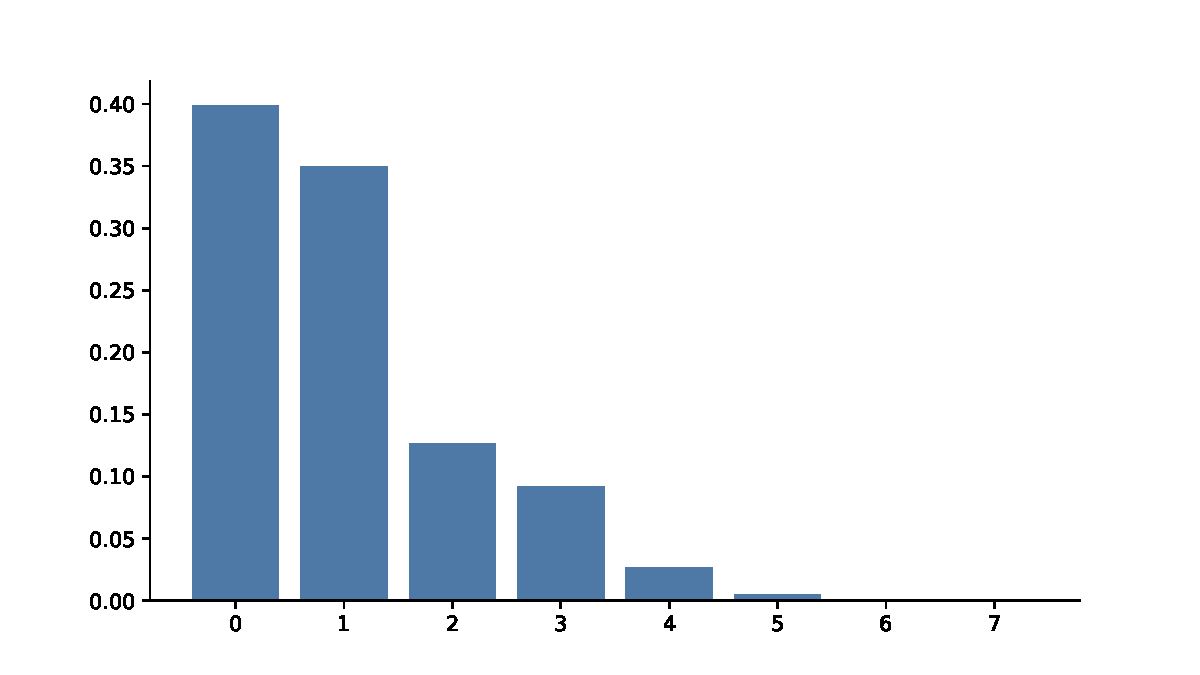
\includegraphics[width=0.5\textwidth]{figures/results/figures/data/distributions_of_the_number_of_contacts/household}
    \caption{Number of Household Contacts}
    \label{fig:n_contacts_hh}
    \floatfoot{\noindent
        \textit{Note:} Every individual meets all other household members every day. The
        German microcensus sampled full households such that our synthetic population
        automatically fits population characteristics such as size and age distribution.}
\end{figure}

\FloatBarrier